\documentclass[sigconf]{acmart}

\settopmatter{printacmref=true, printccs=true}

\usepackage{minted}
\usepackage{siunitx}

\setlength{\marginparwidth}{2cm}
\usepackage{todonotes}
\usepackage{float}
\usepackage{xspace}
\usepackage{mdframed}
\usepackage{stfloats}

%% Using the option "anonymous" will produce "Anonymous Author(s)"
%% for double-anonymized review. Upon acceptance, remove this option
%% and set the authors' names and affiliations using the corresponding
%% commands.

%% CBSoft uses an ACM-like format without the ACM Reference block.
%% The following warning from acmart can be safely ignored:
%% "ACM reference format is mandatory for papers over one page."
\settopmatter{printacmref=false}
\renewcommand\footnotetextcopyrightpermission[1]{} % removes footnote with conference information in first column

%% CBSoft uses an ACM-like format without a copyright note.
\setcopyright{none}

%% These commands are for a PROCEEDINGS abstract or paper.
\acmConference[SBES 2026]{40th Brazilian Symposium on Software Engineering}{September 8–11, 2026}{São Paulo, SP, Brazil}

% CBSoft uses an ACM-like format without CCS Concepts.
% The following warning from acmart can be safely ignored:
% "CCS concepts are mandatory for papers over two pages."

%% \BibTeX command to typeset BibTeX logo in the docs
\AtBeginDocument{
    \providecommand\BibTeX{{Bib\TeX}}
}

%% Only for papers written in PORTUGUESE: 
%% comment out the following three lines
%\renewcommand\abstractname{Resumo}
%\renewcommand\keywordsname{Palavras-chave}
%\renewcommand\refname{Referências}

%% new commands
\newcommand{\ths}{Type Hints\xspace}
\newcommand{\spm}{Structural Pattern Matching\xspace}

%% end of the preamble, start of the body of the document source.


% ------------------------------------------------------------
% Authors: please make sure to read the checklist comments
% provided at the end of this document before submission.
% ------------------------------------------------------------
\begin{document}

%% The "title" command has an optional parameter,
%% allowing the author to define a "short title" to be used on the page 
%% headers.
\title{
Rejuvenation Efforts in Python: \\
A Qualitative Study of Type Hints Adoption
}

%% The "author" command and its associated commands are used to define
%% the authors and their affiliations.
%% Of note is the shared affiliation of the first two authors, and the
%% "authornote" and "authornotemark" commands
%% used to denote shared contribution to the research.
\author{Oseias Magalhães}
\affiliation{
  \institution{Computer Science Department, University of Brasília}
  \city{Brasília}
  \country{Brazil}
}
\email{magalhaes.oseias@aluno.unb.br}

\author{Alana Mota}
\affiliation{
  \institution{Computer Science Department, University of Brasília}
  \city{Brasília}
  \country{Brazil}
}
\email{alana.mota@aluno.unb.br}

\author{Rodrigo Bonifácio}
\affiliation{
  \institution{Informatics Center, Federal University of Pernambuco}
  \city{Brasília}
  \country{Brazil}
}
\email{rbonifacio@cin.ufpe.br}

%% By default, the full list of authors will be used on the page
%% headers. This list is often too long and will overlap
%% other information printed in the page headers. 
%% This command allows the author to define a more concise list
%% of authors' names for this purpose.
\renewcommand{\shortauthors}{Surname1stAuthor et al.}
\renewcommand{\shorttitle}{The Name of the Title Is Hope}

%% The abstract is a short summary of the work the paper presents.

\begin{abstract}
Type Hint modernization has become an important activity in the evolution of Python software as the language and its typing ecosystem continue to evolve. Although previous studies have characterized large-scale code transformations, little is known about the motivations that drive developers to perform these migrations, the practices they adopt, and how they perceive emerging AI-assisted development tools. To investigate these aspects, we conducted a mixed-method empirical study combining repository mining, developer surveys, thematic analysis, and qualitative triangulation. 

Our findings indicate that large-scale Type Hint modernization is driven by the interplay between ecosystem evolution and software quality objectives. Although many modernization campaigns are initiated in response to changes in the Python ecosystem, developers frequently associate these transformations with expected benefits to code quality. Developers predominantly rely on deterministic automation tools, complemented by manual validation, whereas Foundation Models are viewed as useful for semantically complex tasks but are not yet considered suitable replacements for rule-based refactoring. Finally, triangulation between repository artifacts and developer feedback revealed strong semantic agreement, suggesting that repository artifacts provide a useful approximation of developers' motivations, while surveys offer complementary contextual insights.
\end{abstract}


% \begin{abstract}
% \textbf{Context.} Type Hints were introduced in Python as a gradual typing mechanism to enhance code expressiveness without compromising its dynamic nature. With the increasing complexity of large-scale systems and the continuous evolution of the Python ecosystem, this feature has become central to software modernization and quality improvement efforts. \textbf{Aims. }To understand the motivations and practices of developers in large-scale Python code modernization, with a focus on Type Hints and Structural Pattern Matching, based on repository evidence and developer survey data.

% \textbf{Method.} We conducted a mixed-method empirical study combining repository mining, thematic analysis, developer surveys, and qualitative triangulation. We analyzed 141 Python projects, totaling over 674,000 transformations. From this dataset, we selected 117 large-scale commits, for which we collected 20 developer responses via an email survey. The responses were qualitatively analyzed and triangulated with commit messages and pull request discussions to assess semantic alignment across sources.

% \textbf{Results.} Python modernization is primarily driven by software quality and maintainability concerns, including improved readability, bug prevention, and adoption of modern typing practices, particularly Type Hints. Ecosystem-level pressures, such as version deprecation and language evolution, act as secondary drivers that often trigger large-scale transformations.

% These modernization efforts are strongly supported by deterministic automation tools such as \texttt{pyupgrade} and \texttt{ruff}, but still require human validation, especially in large-scale changes. Survey results indicate a predominantly skeptical stance toward the use of large language models (LLMs) for deterministic refactoring tasks, with limited but emerging adoption in semantically complex transformations. Triangulation across commits, pull requests, and developer responses reveals strong semantic alignment across sources.

% \textbf{Conclusion.} Our findings suggest that software modernization in Python is primarily a human-driven process, where developers coordinate and validate automated transformations rather than fully delegating them. Despite the increasing availability of large language models (LLMs), deterministic tools remain the preferred choice for rule-based refactoring tasks due to their reliability and predictability, while LLMs are still mainly used in a limited and supporting role.

% In addition, the strong semantic alignment observed across commits, pull requests, and developer responses indicates that repository artifacts offer valuable insights into developer intent, providing a consistent baseline for studying the motivations behind large-scale code transformations.
%\textbf{Conclusions.} The findings show that Python code modernization is primarily driven by ecosystem evolution pressures, while quality improvements emerge as a consistent secondary effect. Furthermore, development artifacts capture complementary levels of change intent, reinforcing triangulation as a key mechanism for understanding motivations in software evolution. The high semantic alignment observed suggests that, despite heterogeneity across sources, change intent remains largely consistent in the studied ecosystem.
% \end{abstract}

%% Keywords. The author(s) should pick words that accurately describe
%% the presented work. Separate the keywords with commas.
\keywords{Keywords
Software Rejuvenation, Python, Type Hints, Structural Pattern Matching,
Repository Mining, Software Evolution, Refactoring, Developer Survey}

%% This command processes the author, affiliation, and title
%% information and builds the first part of the formatted document.
%% "frenchspacing" avoids an additional space after a period at the end of a sentence.
\frenchspacing
\maketitle

\section{Introduction}
\label{sec:introduction}
% \todo[inline]{TODO: tirar esse foco no artigo anterior logo no começo}

Python has become one of the most widely adopted programming languages due to its flexibility and developer productivity gains~\cite{chun2001core,dyer-fse:2022,malloy-emse:2019,7042702,DBLP:conf/usenix/Rossum07}. However, to remain competitive and suitable for modern software development, Python has continually evolved to incorporate new features. This continuous evolution requires existing code-bases to progressively rejuvenate in order to benefit from newer language capabilities and avoid software aging effects ~\cite{Lucas:jsp2024,Lucas:emse2025,Overbey:regrowing,Pirkelbauer:sc-rejuvenation}. These modernization efforts often involve repository-wide transformations to adopt newer typing syntax, improve compatibility with recent Python versions, simplify type annotations, and leverage advances in static analysis tooling.

To identify representative modernization efforts for qualitative investigation, we build upon a previous large-scale repository mining study that analyzed the evolution history of 141 popular open-source Python projects hosted on GitHub~\cite{refminer}. That study detected more than 674,000 Type Hint-related source code transformations and identified commits containing extensive type-related modifications, providing a rich set of candidate cases for further investigation.

% The results of this previous study revealed a strong predominance of transformations associated with \ths. In addition, the mining process contributed to identifying a subset of large-scale modernization efforts, characterized by commits containing a large volume of automated or semi-automated type-related transformations. These commits are defined as the top-ranked commits in terms of detected refactoring operations, which represent the most intensive modernization efforts observed in the dataset.

% Although the previous study provides a comprehensive quantitative characterization of Python modernization through large-scale mining, it does not explain the underlying decision-making processes that lead developers to perform such extensive transformations. In particular, it does not capture the motivations behind these modifications, the contextual factors influencing modernization decisions, nor the role of developers in orchestrating or validating automated refactoring activities.

To better understand the motivations for those large-scale modernization efforts, we built a curated dataset of 117 representative large-scale commits from an initial set containing the 200 most important commits from each developer. The curation process prioritized commits that best exemplified substantial source code transformations and provided sufficient contextual information for qualitative investigation. A detailed description of this selection procedure is presented in \ref{sec:approach}. Each selected commit was authored by a distinct developer which was used for our subsequent qualitative analysis and developer survey.

Understanding these aspects is essential to complement mining-based studies with evidence that captures developers rationale and the context surrounding modernization efforts. Therefore, in this work, we extend the previous study by investigating the motivations and practices related to large-scale Python modernization.

For this end, we conducted a mixed-method empirical study combining a developer survey with qualitative analysis and triangulation. The survey focused on (i) motivations for performing large-scale \ths-related transformations, (ii) tools and automation techniques used during the process, and (iii) perceptions regarding the potential use of Foundation Models to support software modernization tasks. We analyzed the survey responses using thematic analysis and triangulated the resulting themes with repository artifacts, including commit messages, pull request discussions, and code review comments. This triangulation enabled us to assess the consistency between developer-reported motivations and the evidence observed in the repository history, providing a more comprehensive understanding of large-scale modernization practices.

Overall, this work bridges the gap between large-scale repository mining and a developer-centered understanding of software modernization. Some of the main contributions are:

\begin{itemize}
    \item \textbf{A mixed-method investigation of large-scale Type Hint modernization.} We combine repository mining, developer surveys, thematic analysis, and qualitative triangulation to study the motivations, practices, and perceptions associated with large-scale modernization efforts.

    \item \textbf{An understanding of practices on Type Hints modernization.} We identify the technical and ecosystem-related motivations behind modernization campaigns and characterize the tools and practices developers adopt to perform them.

    \item \textbf{Insights into the emerging role of Foundation Models in software modernization.} We characterize developers' current perceptions of AI-assisted modernization, highlighting both growing acceptance and continued preference for deterministic tooling in rule-based transformations.

    \item \textbf{Evidence supporting the use of repository artifacts as a source of developer rationale.} Through qualitative triangulation, we show that repository artifacts and developer reports are largely consistent, while surveys contribute additional contextual explanations that are often absent from project history.
\end{itemize}

The remainder of this paper is organized as follows. Section \ref{sec:background} provides the background on Python language features and source-code transformations. Section \ref{sec:related-work} reviews the related work. Section \ref{sec:approach} describes the research approach, including the study design, data collection, and analysis procedures. Section \ref{sec:results} presents the results of the empirical study. Section \ref{sec:discussion} discusses the main findings and their implications. Section \ref{sec:threats} outlines the threats to the validity of the study. Finally, Section \ref{sec:conclusion} concludes the paper and discusses directions for future work.

% Python has become one of the most widely adopted programming languages due to its flexibility and developer productivity gains~\cite{chun2001core,dyer-fse:2022,malloy-emse:2019,7042702,DBLP:conf/usenix/Rossum07}. However, to remain competitive and suitable for modern software development, Python, like other programming languages, has continually evolved to incorporate modern features. This continuous evolution requires existing codebases to progressively rejuvenate in order to benefit from newer language capabilities and avoid software aging effects ~\cite{Lucas:jsp2024,Lucas:emse2025,Overbey:regrowing,Pirkelbauer:sc-rejuvenation}.

% Among the most relevant modernization efforts introduced into Python are \ths ~\cite{pep484} and \spm ~\cite{pep634}. The Type Hints, enable developers to incrementally annotate variables, parameters, and return types, improving static analysis, documentation quality, IDE support, and defect detection ~\cite{Khan:type-related-defects,10.1145/3540250.3549114}.  Structural Pattern Matching, extends the language with declarative pattern-based control flow using the \texttt{match/case} construct, allowing developers to replace traditional \texttt{if-elif-else} chains with more expressive and maintainable structures.  Together, these features represent important steps toward modernizing Python systems and improving software comprehensibility and maintainability over time.

% Although previous studies have investigated the adoption and benefits of Type Hints and Structural Pattern Matching ~\cite{10.1145/3540250.3549114,Khan:type-related-defects,10006855,10589769}, important aspects of their evolutionary adoption process remain underexplored. Existing research has mainly focused on static snapshots of adoption or code quality benefits, with limited attention given to how developers modernize legacy Python systems over time.

% To address these gaps, this paper investigate software rejuvenation practices in Python projects through the analysis of source-code transformations related to \ths and \spm. To achieve this goal, we extended the RefactoringMiner infrastructure ~\cite{refminer} and mined the evolution history of 141 popular open-source Python projects hosted on GitHub, collecting more than 674,000 transformation instances. Some of our
% findings are:


\section{Background}
\label{sec:background}
% \todo[inline, color=green]{Talvez reescrever um pouco. Diria que duas modernizações relevantes sob a perspectiva de melhorar a legibilidade de código e no caso de possibilitar a detecção de erros de tipos via a integração de ferramentas de análise estática \ldots. Como \spm não são tão usadas, acho que relevante é muito forte.}
% \todo[inline, color=green]{Acho que ao longo desta seção II, deveríamos contextualizar a pesquisa anterior, e deixar claro que esse trabalho de Iniciação Científica se aprofundou para explorar aspectos qualitativos não investigados no trabalho anterior. Apesar disso já ter sido discutido na introdução, é super inportante reforçar aqui em Background.}
% \todo[inline]{Em todo o texto, sempre que possível eu utilizaria o termo transformation ou source code transformation, no lugar de refactoring.}

Python has continuously evolved by introducing language features intended to improve software maintainability and supporting large-scale software development. Among these, \ths were introduced to improve code readability, standardize the specification of type information, and enable the detection of type-related issues through integration with static analysis tools. In our previous work, we quantitatively investigated large-scale \ths adoption by mining software repositories and identifying commits involving extensive type-related source code transformations. Although that study characterized how these transformations occur in practice, it did not investigate the motivations, decision-making processes, or development practices underlying them. This paper extends that work through a qualitative, developer-centered investigation based on survey responses and artifact triangulation.

\subsection{Type Hints}\label{subsec:ths}

Type Hints were standardized in PEP 484~\cite{pep484} as part of Python's gradual typing system to address the lack of a standardized mechanism for expressing type information in Python programs. Prior to their adoption, developers relied on heterogeneous approaches, including decorators, docstrings, and conventions implemented by third-party libraries, resulting in incompatible annotation styles and limited interoperability among tools~\cite{pep3107}. This lack of standardization also hindered IDE support and automated source code transformation capabilities.

PEP 484 established a common vocabulary for annotating function parameters, return types, and variables, enabling external tools to perform offline static analysis while preserving Python's dynamically typed nature~\cite{pep484}. Subsequent proposals, including PEP 526~\cite{pep526} and PEP 585~\cite{pep585}, extended typing support by introducing native variable annotations and built-in generic types. In particular, PEP 526 replaced comment-based annotations (e.g., \texttt{\# type: annotation}), which suffered from readability limitations, artificial variable initializations, and poor accessibility for automated tools~\cite{pep526}.

Unlike statically typed languages, Python does not use type annotations during runtime. Instead, they provide semantic information for external tools such as MyPy and Pyright, which exploit them for offline static analysis, code completion, navigation, and automated source code transformations~\cite{pep484}. Previous work also reports benefits including earlier bug detection, improved software quality, and better software maintenance activities~\cite{10.1145/3426422.3426981}. Importantly, Type Hints remain entirely optional, preserving Python's dynamically typed execution model while enabling optional analysis and validation by external tools and libraries~\cite{pep484,pep526}, as illustrated in Figure~\ref{lst:pep484_greeting}.

\begin{listing}[h]
\caption{Example of a function with Type Hints in Python (PEP 484~\cite{pep484}).}
\label{lst:pep484_greeting}

\begin{minted}[frame=single, fontsize=\small]{python}
def greeting(name: str) -> str:
    return 'Hello ' + name
\end{minted}
\end{listing}
% \ths were standardized in PEP 484~\cite{pep484} as part of Python's gradual typing system. They allow developers to incrementally annotate variables, function parameters, and return types with optional type information, enabling static analysis and improving maintainability. Additional proposals, such as PEP 526~\cite{pep526} and PEP 585~\cite{pep585}, further extended typing support by introducing variable annotations and built-in generic types.

% \todo[inline]{Também tomaria cuidado com essa expressão 'type-checking at runtime'. Python faz verificação de tipos em tempo de execução, não estaticamente. Talvez indicar que as anotações de tipos não são consideradas em tempo de execução. Concordam? Podemos discutir isso amanhã.}

% Unlike statically typed languages, Python does not enforce type checking at runtime. Instead, type annotations are mainly used by external tools such as MyPy and Pyright to support static analysis, autocompletion, and error detection. Prior studies also suggest that type hints can improve software quality and maintenance activities~\cite{10.1145/3426422.3426981}.

%\subsection{Structural Pattern Matching}\label{subsec:spm}

% \spm was introduced in Python 3.10 through PEP 634~\cite{pep634}. The feature extends Python with the \texttt{match/case} construct, allowing developers to express conditional logic through structural patterns rather than traditional \texttt{if-elif-else} chains.

% Besides improving readability, \spm enables declarative inspection and deconstruction of structured data, supporting patterns such as literals, sequences, and guarded expressions~\cite{10.1145/3426422.3426983}.% Figure~\ref{fig:spm_examples} illustrates examples of value matching and structural decomposition using \texttt{match/case}.

% \begin{figure}[htb]
% \centering
% \begin{minipage}[t]{0.48\textwidth}
% \begin{minted}[fontsize=\scriptsize, frame=single]{python}
% def fact(arg: int) -> int:
%     match arg:
%         case 0 | 1:
%             f: int = 1
%         case n:
%             f: int = n * fact(n - 1)
%     return f
% \end{minted}
% \centering
% \scriptsize (a) Pattern matching example for factorial
% \end{minipage}
% \hfill
% \begin{minipage}[t]{0.48\textwidth}
% \begin{minted}[fontsize=\scriptsize, frame=single]{python}
% def sum(seq):
%     match seq:
%         case []:
%             s = 0
%         case [hd, *tl]:
%             s = hd + sum(tl)
%     return s
% \end{minted}
% \centering
% \scriptsize (b) Structural deconstruction using \spm
% \end{minipage}
% \caption{Examples of Structural Pattern Matching in Python.}
% \Description{
% Examples of Structural Pattern Matching in Python showing factorial
% computation and recursive list summation.
% }
% \label{fig:spm_examples}
% \end{figure}

\subsection{Program Transformations}
\label{subsec:transformations}

In this study, we investigate source code transformations involving Python type annotations. These transformations include the introduction, removal, and modification of type annotations in variables, function parameters, and return types, reflecting how developers evolve typing information as projects adopt modern Python features. By analyzing these transformations, we investigate the motivations, practices, and decision-making processes underlying large-scale software modernization.

% We also analyze transformations involving \spm, particularly the replacement of traditional \texttt{if-elif-else} chains with \texttt{match/case} constructs, and the reverse operation. Such transformations reflect modernization efforts aiming to improve readability and maintainability of conditional logic.

%In addition to fine-grained transformations, we derive function-level annotation completeness categories, distinguishing between fully annotated signatures and partially annotated functions. These categories help characterize the gradual adoption process of typing information in Python projects.

\subsection{Large-Scale Modernization}
\label{subsec:large-scale-modernization}

% As an illustrative example of a large-scale modernization effort, we inspected commit \texttt{9c8557a} from the \texttt{chia-blockchain} project, which contains 6,421 detected type-related transformations. This is the largest commit in the dataset we built in our previous work, and alone accounts for 6.47\% of all detected transformations. The commit corresponds to a systematic migration of legacy type annotations from the \texttt{typing} module to the built-in generic types introduced in Python 3.9 (PEP 585 \cite{pep585}).

% The changes were performed consistently across the codebase and primarily involve replacing legacy constructs such as \texttt{List}, \texttt{Dict}, and \texttt{Tuple} with their built-in counterparts (\texttt{list}, \texttt{dict}, and \texttt{tuple}). This example illustrates how Python modernization efforts may be conducted through large-scale refactoring campaigns affecting thousands of annotation occurrences within a single commit.

Large-scale modernization refers to systematic source code transformations that affect many locations across a codebase within a single development effort. Such transformations are commonly associated with software reengineering and automated program transformation, particularly when their scale makes manual application impractical\cite{AKERS2007275}. These efforts may be motivated by the adoption of newer language features, improvements in code quality, and keep projects aligned with the evolution of the programming language. Figure~\ref{fig:modernization-example} illustrates a representative example from the \texttt{aiohttp} project (commit 35754d4), where type annotations were consistently updated across the repository by replacing legacy typing constructs with their modern counterparts, such as migrating generic types introduced by PEP 585~\cite{pep585}, simplifying optional types using PEP 604~\cite{pep604}, and updating imports according to current Python recommendations. This example highlights how software modernization is often performed through coordinated, repository-wide transformations.

% \todo[inline, color=green]{Talvez fosse mais interessante mostrar um diff de uma parte pequena do código, em vez desta tabela. O artigo anterior deve ter um exemplo.}


\begin{figure}[H]
\begin{minted}[fontsize=\small]{diff}
--- a/aiohttp/_cookie_helpers.py    (Python 3.8 style)
+++ b/aiohttp/_cookie_helpers.py    (Python 3.9+ style)
@@ -6,6 +6,7 @@
import re
+from collections.abc import Sequence
from http.cookies import Morsel
-from typing import List, Optional, Sequence, Tuple, cast
+from typing import cast

@@ -159,9 +160,9 @@
def parse_cookie_header(header: str) ->
-   List[Tuple[str, Morsel[str]]]:
+   list[tuple[str, Morsel[str]]]:
     ...                                                                         
-    cookies: List[Tuple[str, Morsel[str]]] = []
+    cookies: list[tuple[str, Morsel[str]]] = []
       ...
-    current_morsel: Optional[Morsel[str]] = None
+    current_morsel: Morsel[str] | None = None
\end{minted}
\caption{Python type annotation modernization in \texttt{aiohttp} (commit \texttt{35754d4}).}
\label{fig:modernization-example}
\end{figure}

% Table~\ref{tab:chia_commit} summarizes the most frequent transformations identified in this commit.

% \begin{table}[htb]
% \caption{Most frequent type annotation transformations in commit \texttt{9c8557a} (\texttt{chia-blockchain}).}
% \label{tab:chia_commit}
% \centering
% \begin{tabular}{lrr}
% \toprule
% \textbf{Transformation} & \textbf{Removed} & \textbf{Added} \\
% \midrule
% \texttt{List} $\rightarrow$ \texttt{list}   & 2,820 & 2,822 \\
% \texttt{Dict} $\rightarrow$ \texttt{dict}   & 1,839 & 1,840 \\
% \texttt{Tuple} $\rightarrow$ \texttt{tuple} & 1,080 & 1,082 \\
% \bottomrule
% \end{tabular}
% \end{table}

\subsection{Foundation Models}
\label{subsec:foundation-models}

Foundation models are large-scale machine learning models trained on broad and diverse datasets and designed to support a wide range of downstream tasks through adaptation or direct use~\cite{DBLP:journals/corr/abs-2108-07258}. Unlike models developed for a single predefined task, foundation models provide general-purpose capabilities that can be reused across different application domains. Recent advances in the scale of training data, model architectures, and computational resources have enabled foundation models to perform increasingly diverse tasks involving natural language, code, images, and other modalities.

In software development, foundation models trained on source code and natural language have enabled new forms of programming assistance, including code generation, code completion, explanation, summarization, and source code transformation. Large language models (LLMs) are a prominent class of foundation models that can process and generate natural language and programming languages, allowing developers to interact with them using natural-language instructions. These capabilities have introduced new possibilities for automating or assisting software engineering activities, while still requiring developers to validate and integrate the generated results into existing development workflows.


\section{Related Work}
\label{sec:related-work}
Software rejuvenation refers to the process of updating legacy codebases to incorporate modern programming language features while preserving their original semantics ~\cite{DBLP:conf/sofsem/PirkelbauerDS10}. Unlike general refactoring, which focuses on improving internal structure, rejuvenation addresses technical obsolescence driven by language evolution and ecosystem changes. Prior work has highlighted that such modernization efforts often involve trade-offs between adopting new language features and maintaining backward compatibility in existing systems~\cite{mendonca2026}.

Empirical studies on Python evolution have primarily focused on the adoption of specific language features. Research on type hints shows that their adoption initially emerged at low rates and is typically partial, often concentrated on function signatures rather than full codebases ~\cite{10.1145/3426422.3426981, 10.1145/3540250.3549114}. Once introduced, type annotations tend to remain stable over time, with adoption largely motivated by improved documentation and tool support such as static analysis and IDE assistance ~\cite{asarethird2026}.

%Similarly, studies on \spm have investigated its impact on code structure and readability. Results indicate that \texttt{match/case} constructs can reduce syntactic complexity compared to traditional conditional chains, although their benefits may vary depending on usage context and developer familiarity~\cite{10006855, 10589769}.

While existing studies have primarily focused on adoption rates, automated transformations, or language design, fewer works investigate the motivations behind large-scale code modernization from the developer’s perspective. Some recent efforts have begun to incorporate qualitative analysis of development artifacts to better understand intent behind changes~\cite{DBLP:conf/sbqs/CarvalhoB0M24}. However, these studies still rarely combine repository mining with direct developer feedback.

In contrast, this study investigates the motivations behind software rejuvenation in Python systems by combining repository mining with thematic analysis and triangulation of commit messages, pull requests, and developer responses. This enables a complementary perspective that connects observable code changes with the underlying intentions expressed by developers.


\section{Approach}
\label{sec:approach}

\begin{figure*}[!t]
    \centering
    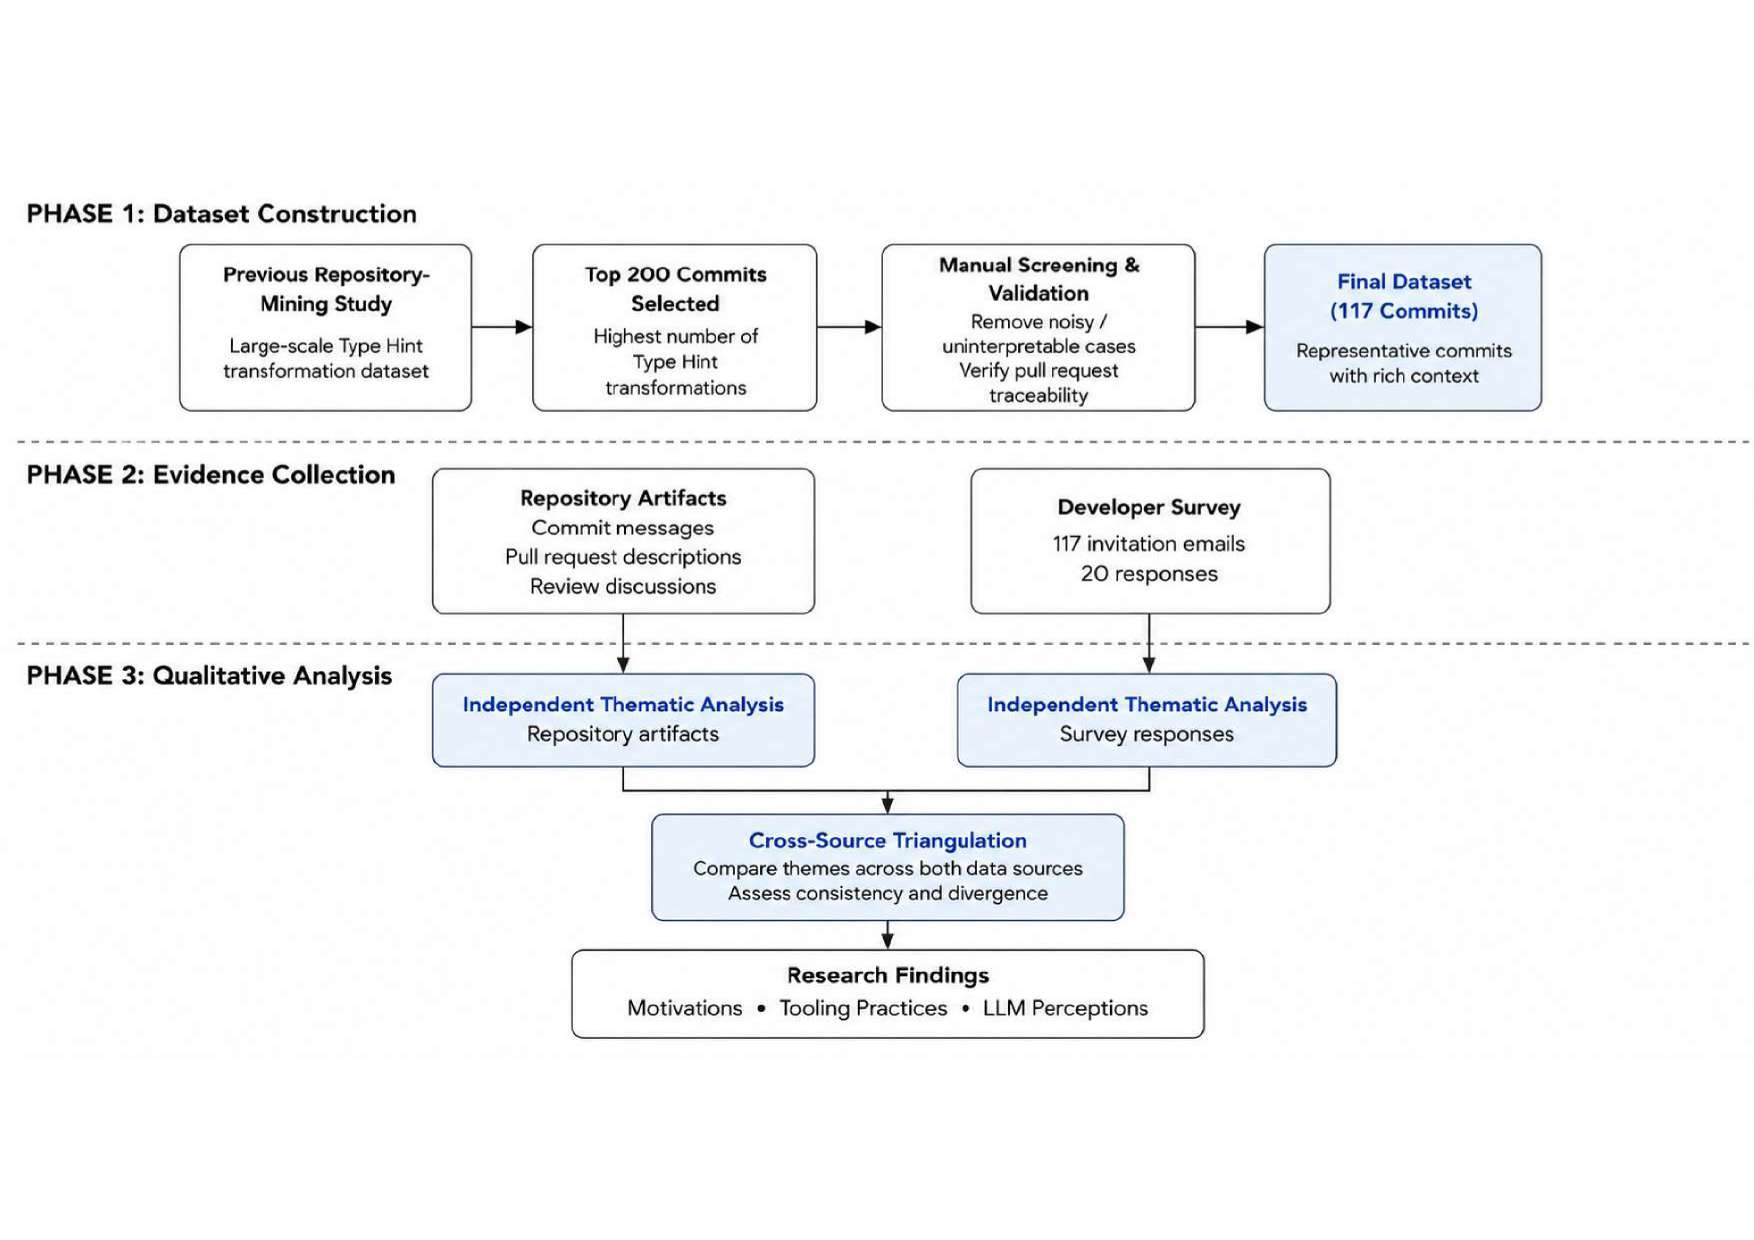
\includegraphics[width=\textwidth]{imgs/metodologia_horizontal.pdf}
    \caption{Overview of the research methodology.}
    \label{fig:methodology}
\end{figure*}

This study investigates the motivations and practices associated with large-scale Python modernization efforts involving \ths. Figure~\ref{fig:methodology} presents an overview of the research workflow. While our previous research (based on a large-scale repository-mining analysis) characterizes how these transformations occur, it does not reveal the reasoning behind developers' decisions, the role of automation in modernization, or developers' perspectives on emerging AI-based support. To address these aspects, we conducted a survey with authors of commits containing a large number of detected type-related transformations.

Specifically, we aim to understand why developers introduce and evolve type annotations, whether they rely on tools to support such modifications, and how they perceive the potential use of Foundation Models for similar tasks. To guide this investigation, we address the following research questions:

\begin{itemize}
\item \textbf{RQ1: What motivations drive developers to perform large-scale Type Hint modernization efforts?} This question investigates the related factors that motivate developers to modernize Type Hints across large open-source Python projects.

\item \textbf{RQ2: What tools or automation techniques do developers use to support large-scale Type Hint modifications?} This question investigates the tools, scripts, and automation strategies developers employ to facilitate large-scale Type Hint modernization.

\item \textbf{RQ3: How do developers perceive the potential use of Foundation Models to assist Type Hint modernization tasks?} This question seeks to identify developers' expectations, perceived benefits, concerns, and potential use cases for applying to Type Hint modernization.
\end{itemize}

We analyze survey responses using thematic analysis and integrate these findings with evidence extracted from commits and pull request discussions. We then perform a triangulation of evidence across the three sources (commits, pull requests, and survey responses), assessing consistency between observed code changes and developers’ reported motivations and practices.

This triangulation enables a more comprehensive understanding of large-scale \ths modernization by connecting observable software evolution with developer intent and decision-making processes.

\subsection{Study Settings}

We build upon a large-scale mining dataset of 141 popular Python repositories, selecting the top 200 commits with the highest number of \ths-related transformations. From this set, we manually curate a final dataset of 57 projects and 117 representative commits based on their relevance and the richness of contextual information available in the associated pull requests.

For each selected commit, we retrieve and analyze the corresponding pull request discussions when available. In cases where no pull request was explicitly linked, we manually verify the repository history to ensure traceability. Each commit is associated with a single primary pull request, and this relationship was validated manually.

To complement repository analysis, we contacted the authors of the 117 selected commits via email. Although 10 developers were unreachable, we obtained 20 valid responses from 20 different projects. The survey is exploratory in nature and aims to capture developers’ perspectives on motivations, tooling practices, and the potential use of Foundation Models in modernization tasks.

\subsection{Data Collection}

\subsubsection{Commit Selection}

Starting from the dataset produced in our previous study, we identified candidate commits according to two criteria: (i) the number of detected type-related source code transformations and (ii) recency, considering commits authored between 2024 and 2026. This subset accounts for 39.43\% of all detected transformations. To avoid over representing highly active contributors, we retained only the commit containing the largest number of detected transformations for each developer, ensuring that each developer was represented only once. These commits represent 24.28\% of transformations within the selected time period. We then excluded commits associated with GitHub \textit{noreply} accounts, since their authors could not be reliably contacted for the survey. The remaining commits were ranked according to their number of detected transformations then we selected the top 200, this subset covers 58.37\% of all transformations in the developers' largest commits during the selected period. Providing a manageable yet highly representative sample for the subsequent qualitative analysis.

\subsubsection{Survey Procedure}

We manually inspected each of the selected commits to assess whether the detected transformations were sufficiently evident and interpretable for a follow-up developer survey. Commits containing numerous unrelated modifications, where the detected transformations were part of broader code changes and their rationale could not be reliably inferred, were excluded. We also discarded cases lacking sufficient contextual information (e.g., commit messages or associated pull requests discussions) to support the qualitative analysis and survey design. This manual screening resulted in a final dataset of 117 commits.

We contacted the authors of the 117 selected commits through an e-mail survey containing the questions presented in Table~\ref{tab:survey_questions}. The questionnaire investigated (i) the motivations behind the transformations, (ii) the tools and automation practices adopted during the modernization process, and (iii) developers' perceptions regarding the use of language models for similar tasks.

\begin{table}[htb]
\caption{Script of the survey questions}
\label{tab:survey_questions}
\centering
\begin{tabular}{p{0.05\linewidth} p{0.80\linewidth}}
\toprule
\textbf{RQ} & \textbf{Question} \\
\midrule
RQ1 &
What was your decision-making process and rationale for introducing this change? \\

RQ2 &
Did you use any tools or automation to support this large-scale modification? \\

RQ3 &
Do you envision using language models to assist with this kind of task? \\
\bottomrule
\end{tabular}
\end{table}

Overall, we received 20 responses (17.09\% response rate), each from different open-source Python projects. The respondents include developers from widely used projects such as \textit{FastAPI}, \textit{aiohttp}, \textit{Scrapy}, \textit{MyPy}, \textit{Pipenv}, \textit{Locust} and \textit{Chia Blockchain}, including spanning domains. This diversity widens the range of perspectives captured.

\subsubsection{Repository Artifact Collection}

For each of the 20 survey responses, we collected the corresponding repository artifacts to support a triangulated analysis of software development decisions. Each case was anchored on a surveyed commit and expanded using the GitHub API to retrieve all associated contextual artifacts.

Specifically, we retrieved commit messages, pull request descriptions, and review-related discussions. Pull request data was obtained using the \texttt{/commits/{sha}/pulls} endpoint, while additional discussion context was collected using the issues and pull request review APIs, including issue comments (\texttt{/issues/{number}/comments}), review comments (\texttt{/pulls/{number}/comments}), and structured review events (\texttt{/pulls/{number}/reviews}). Consequently, each case in the dataset consists of multiple complementary sources of evidence: the developer's survey response, the associated commit message, the pull request description, and the corresponding review and discussion artifacts.

To construct each triangulated case, all artifacts were grouped by their associated commit and pull request identifiers, ensuring that all related discussion and review data were aggregated into a single analytical unit. This allowed us to capture both implementation-level decisions and the surrounding design rationale expressed during the review process.

To support qualitative analysis, the first two authors independently recorded observations for each case. For each artifact type, separate notes were produced summarizing the technical motivations, design considerations, and decision-making rationale expressed by developers across commits, pull requests, and review discussions.

\subsection{Data Analysis}
\label{subsec:data-analysis}

To investigate developers’ decision-making processes behind large-scale code changes, the use of tools and automation during these modifications, and their perceptions regarding the use of large language models (LLMs) to support such tasks, we analyzed 20 survey responses using thematic analysis following Braun and Clarke~\cite{Braun01012006}.

The unit of analysis consisted of two complementary data sources: (i) textual excerpts extracted from commits, pull request descriptions, and code review comments, and (ii) developers’ survey responses. Both sources were analyzed separately using thematic analysis. These excerpts were manually coded at a fine-grained level using a multi-label coding scheme, in which multiple codes could be assigned to the same segment when appropriate. The coding was performed explicitly, without inferring categories not directly supported by the text. Although most codes emerged from the data, some initial categories were informed by prior literature and were subsequently refined throughout the analysis process. Excerpts considered irrelevant according to predefined criteria—such as purely social interactions or comments without technical implications—were excluded from coding.

Following Braun and Clarke’s guidelines, the analysis proceeded through iterative cycles of data familiarization, code generation, grouping related codes into candidate themes, and continuous refinement until a stable thematic structure was achieved. Rather than following a strictly linear pipeline, the coding and theme refinement process was revisited multiple times to ensure consistency and conceptual coherence. The process was conducted in pairs, with independent coding by two researchers followed by comparison and reconciliation of differences. This cross-validation process helped increase consistency and reduce individual interpretation bias.

We also followed established practices for trustworthiness in qualitative research, including triangulation of interpretations between researchers, discussion meetings among researchers (peer debriefing), debate of individual perspectives during the analysis, investigator triangulation, and cross-checking of coding decisions until reaching consensus among the researchers~\cite{Nowell2017Trustworthiness}.

We used ATLAS.ti~\cite{atlas_ti} to support data organization, coding management, and traceability of analytical decisions, enabling an audit trail of code evolution and theme refinement. This contributed to the transparency and reliability of the analytical process.

Overall, the resulting themes characterizing developers’ motivations, modernization practices, and perceptions of AI-assisted transformations are presented in Section~\ref{sec:results}.


\subsection{Triangulation}

For each of the 20 cases, we performed a qualitative triangulation of developer intent by comparing the results of two thematic analyses: one conducted on repository artifacts (commit messages, pull request descriptions, and code review comments) and another conducted on survey responses. Each case corresponded to a single commit, its associated pull request and review discussion, and the corresponding developer survey response, treated as a unified unit of analysis.

The themes identified through thematic analysis were compared across these sources without re-coding the data, focusing on whether the same underlying motivation was expressed across different artifacts. This comparison assessed the degree of consistency between developers’ reported motivations and the motivations observed in repository artifacts.

Consistency was evaluated qualitatively based on the extent to which motivations converged across sources, considering both alignment and partial divergence in emphasis or detail.

This process was conducted independently by two researchers, and disagreements in interpretation were resolved through discussion until consensus was reached.

% % \todo[inline]{
% % TODO: reescrever o approach\\
% % - reasearch questions deve estar mais relacionadas as perguntas feitas aos devs\\
% % - explicar os parâmetros para coleta \\
% % - explicar como foi feito a analise temática\\
% % - referenciar commits que são exemplos de grandes refatorações em um único commit
% % }

% % \todo[inline, color = green]{Esse próximo parágrafo dá a entender que é só type-hints. Não vejo problema com isso, mas, se for desta forma, melhor revisar todo o texto para excluir structural pattern matching.}
% % \todo[inline, color=green]{E novamente, esse parágrafo também indica que a pesquisa se concentrou apenas em survey, mas outros pontos do texto fala em triagulação, análise de PRs, \ldots. Precisamos manter consistência no artigo.}

% \todo[inline]{adicionar iamgem da metodologia}
% % \begin{figure*}[t]
% % \centering
% % \includegraphics[width=\textwidth,height=0.35\textheight,keepaspectratio]{imgs/methodology.jpeg}
% % \caption{Overview of the research methodology, combining repository-based analysis, developer survey, and triangulation across multiple artifacts.}
% % \Description{A workflow diagram showing the research process. It starts with repository mining of Python projects, followed by ranking and selecting commits, manual curation to 117 commits, and branching into two paths: repository-based analysis (pull request analysis and commit-PR validation) and developer survey (data collection, responses, and thematic analysis). Both branches converge into a triangulation step that integrates commits, pull requests, and survey responses to assess consistency.}
% % \label{fig:methodology}
% % \end{figure*}

% This study investigates the motivations and practices associated with large-scale Python modernization efforts involving \ths. Figure~\ref{fig:methodology} presents an overview of the research workflow. While our previous research (based on a large-scale repository-mining analysis) characterizes how these transformations occur, it does not reveal the reasoning behind developers' decisions, the role of automation in modernization, or developers' perspectives on emerging AI-based support. To address these aspects, we conducted a survey with authors of commits containing a large number of detected type-related transformations.


% % \todo[inline, color=green]{Acho mais interessante o termo Foundation Models, em vez de large language models. Revisar em todo o artigo. Nem todo modelo de linguagem é de grande escala.}

% Specifically, we aim to understand why developers introduce and evolve type annotations, whether they rely on tools to support such modifications, and how they perceive the potential use of Foundation Models for similar tasks. To guide this investigation, we address the following research questions:

% \begin{itemize}
% \item \textbf{RQ1: What motivations drive developers to perform large-scale Type Hint modernization efforts?} This question investigates the related factors that motivate developers to modernize Type Hints across large open-source Python projects.

% \item \textbf{RQ2: What tools or automation techniques do developers use to support large-scale Type Hint modifications?} This question investigates the tools, scripts, and automation strategies developers employ to facilitate large-scale Type Hint modernization.

% \item \textbf{RQ3: How do developers perceive the potential use of Foundation Models to assist Type Hint modernization tasks?} This question seeks to identify developers' expectations, perceived benefits, concerns, and potential use cases for applying to Type Hint modernization.
% \end{itemize}

% Our study follows a mixed-method design. First, we build upon a large-scale mining dataset of Python repositories and select the top 200 commits with the highest number of \ths-related transformations. From this set, we manually curate a final dataset of 117 representative commits based on their relevance and the richness of contextual information available in associated pull requests.

% For each selected commit, we retrieve and analyze the corresponding pull request discussions when available. In cases where no pull request was explicitly linked, we manually verify repository history to ensure traceability. Each commit is associated with a single primary pull request, and this relationship was validated manually.

% To complement repository analysis, we contacted the authors of the 117 selected commits via email. Although 9 developers were unreachable, we obtained 20 valid responses. The survey is exploratory in nature and aims to capture developers’ perspectives on motivations, tooling practices, and the potential use of Foundation Models in modernization tasks.

% We analyze survey responses using thematic analysis and integrate these findings with evidence extracted from commits and pull request discussions. We then perform a triangulation of evidence across the three sources (commits, pull requests, and survey responses), assessing consistency between observed code changes and developers’ reported motivations and practices.

% This triangulation enables a more comprehensive understanding of large-scale \ths modernization by connecting observable software evolution with developer intent and decision-making processes.

% \subsection{Data Collection}
% \label{subsec:data-collection}

% % \todo[inline, color=green]{Importante reforçar não apenas os procedimentos do survey.}

% \subsubsection{Commit Selection}
% To complement the quantitative findings of our previous study, we collected qualitative evidence from multiple complementary sources, including repository artifacts (commits and pull requests) and a developer survey. Rather than relying solely on developers response, we combined the survey data with repository artifacts to enable triangulation between observed code changes and developers’ reported motivations and practices.

% Starting from the dataset produced in our previous study, we identified candidate commits according to two criteria: (i) the number of detected type-related source code transformations and (ii) recency, considering commits authored between 2024 and 2026. This subset accounts for 39.43\% of all detected transformations. To avoid over representing highly active contributors, we retained only the commit containing the largest number of detected transformations for each developer, ensuring that each developer was represented only once. These commits represent 24.28\% of transformations within the selected time period. We then excluded commits associated with GitHub \textit{noreply} accounts, since their authors could not be reliably contacted for the survey. The remaining commits were ranked according to their number of detected transformations then we selected the top 200, this subset covers 58.37\% of all transformations in the developers' largest commits during the selected period. Providing a manageable yet highly representative sample for the subsequent qualitative analysis.

% % For each selected commit, we retrieved and analyzed the corresponding pull request when available, ensuring traceability between implementation changes and their documented rationale. In cases where no pull request was explicitly linked, we manually inspected repository history to recover the most relevant contextual discussion.

% % Only after this full artifact-based filtering process did we contact developers via email to conduct the survey. After removing 9 unreachable contacts, we obtained 20 valid responses. These responses were then analyzed in conjunction with commit and pull request data as part of our triangulation strategy.

% % \todo[inline]{Tem que ajustar o parágrafo anterior com esse. Em alguns pontos, está dando a impressão que o survey é a fonte principal. Ela é super importante, mas as análises manuais de commits e PRs também são relevantes para a triangulação. }
% % \todo[inline]{Talvez incluir uma figura com cada passo para a construção do conjunto final. Iniciou com 200, aplicou um filtro que reduziu para ABC, outro filtro que, até chegar em 117 commits. Os parágrafos a seguir se concentram no survey. Seria legal enfatizat tudo.}

% % Next, we manually inspected the source-code changes and commit messages associated with each selected commit. The goal was to identify commits that best represented large-scale modernization efforts and provided sufficient context to answer our research questions. This curation process resulted in a final dataset of 117 commits.

% \subsubsection{Survey Procedure}
% We manually inspected each of the selected commits to assess whether the detected transformations were sufficiently evident and interpretable for a follow-up developer survey. Commits containing numerous unrelated modifications, where the detected transformations were part of broader code changes and their rationale could not be reliably inferred, were excluded. We also discarded cases lacking sufficient contextual information (e.g., commit messages or associated pull requests discussions) to support the qualitative analysis and survey design. This manual screening resulted in a final dataset of 117 commits.

% We contacted the authors of the 117 selected commits through an e-mail survey containing the questions presented in Table~\ref{tab:survey_questions}. The questionnaire investigated (i) the motivations behind the transformations, (ii) the tools and automation practices adopted during the modernization process, and (iii) developers' perceptions regarding the use of language models for similar tasks.

% \begin{table}[htb]
% \caption{Script of the survey questions}
% \label{tab:survey_questions}
% \centering
% \begin{tabular}{p{0.05\linewidth} p{0.80\linewidth}}
% \toprule
% \textbf{RQ} & \textbf{Question} \\
% \midrule
% RQ1 &
% What was your decision-making process and rationale for introducing this change? \\

% RQ2 &
% Did you use any tools or automation to support this large-scale modification? \\

% RQ3 &
% Do you envision using language models to assist with this kind of task? \\
% \bottomrule
% \end{tabular}
% \end{table}

% Overall, we received 20 responses (17.09\% response rate), each from different open-source Python projects. The respondents include developers from widely used projects such as \textit{FastAPI}, \textit{aiohttp}, \textit{Scrapy}, \textit{MyPy}, \textit{Pipenv}, \textit{Locust} and \textit{Chia Blockchain}, including spanning domains. This diversity widens the range of perspectives captured.

% \subsubsection{Repository Artifact Collection}

% For each of the 20 survey responses, we collected the corresponding repository artifacts to support a triangulated analysis of software development decisions. Each case was anchored on a surveyed commit and expanded using the GitHub API to retrieve all associated contextual artifacts.

% Specifically, we retrieved commit messages, pull request descriptions, and review-related discussions. Pull request data was obtained using the \texttt{/commits/\{sha\}/pulls} endpoint, while additional discussion context was collected using the issues and pull request review APIs, including issue comments (\texttt{/issues/\{number\}/comments}), review comments (\texttt{/pulls/\{number\}/comments}), and structured review events (\texttt{/pulls/\{number\}/reviews}). Consequently, each case in the dataset consists of multiple complementary sources of evidence: the developer's survey response, the associated commit message, the pull request description, and the corresponding review and discussion artifacts.

% To construct each triangulated case, all artifacts were grouped by their associated commit and pull request identifiers, ensuring that all related discussion and review data were aggregated into a single analytical unit. This allowed us to capture both implementation-level decisions and the surrounding design rationale expressed during the review process.

% To support qualitative analysis, the first two authors independently recorded observations for each case. For each artifact type, separate notes were produced summarizing the technical motivations, design considerations, and decision-making rationale expressed by developers across commits, pull requests, and review discussions.

% % We selected popular and actively maintained Python repositories hosted on GitHub using the SEART tool~\cite{Dabic2021}, following criteria inspired by previous mining studies~\cite{Zampetti2024}. The initial selection considered repositories that: (i) use Python as the primary language, (ii) are not forks, (iii) contain at least 1,000 commits, and (iv) have at least 10,000 stars. We additionally required recent maintenance activity within 90 days prior to data collection (April 2026).

% % We further refined the dataset by retaining only repositories with at least 10 branches, 30 contributors, and 100 forks. After manually removing tutorial-style and educational repositories, the final dataset comprised 141 projects.

% % We mined the complete commit history of each repository from January 2015 onward using our RefactoringMiner extension. The mining process was executed in batches to avoid memory limitations in large repositories and parallelized at the project level. After collection, the results were filtered to retain only transformations occurring in Python source files.

% % Overall, the resulting dataset contains more than 674,000 transformations across 127 repositories with at least one detected modernization instance.

% \subsection{Thematic Analysis}
% \label{subsec:thematic-analysis}
% % \todo[inline, color=green]{Citar o trabalho de Braun e Clarke. Essa seção não está muito bem escrita. O texto está todo na voz passiva, enquanto que o restante do artigo está na voz ativa. Parece uma lista de bullets. Acho que pode melhorar. }

% To investigate developers’ decision-making processes behind large-scale code changes, the use of tools and automation during these modifications, and their perceptions regarding the use of large language models (LLMs) to support such tasks, we analyzed 20 survey responses using thematic analysis following Braun and Clarke~\cite{Braun01012006}.

% The unit of analysis consisted of two complementary data sources: (i) textual excerpts extracted from commits, pull request descriptions, and code review comments, and (ii) developers’ survey responses. Both sources were analyzed separately using thematic analysis. These excerpts were manually coded at a fine-grained level using a multi-label coding scheme, in which multiple codes could be assigned to the same segment when appropriate. The coding was performed explicitly, without inferring categories not directly supported by the text. Although most codes emerged from the data, some initial categories were informed by prior literature and were subsequently refined throughout the analysis process. Excerpts considered irrelevant according to predefined criteria—such as purely social interactions or comments without technical implications—were excluded from coding.

% Following Braun and Clarke’s guidelines, the analysis proceeded through iterative cycles of data familiarization, code generation, grouping related codes into candidate themes, and continuous refinement until a stable thematic structure was achieved. Rather than following a strictly linear pipeline, the coding and theme refinement process was revisited multiple times to ensure consistency and conceptual coherence. The process was conducted in pairs, with independent coding by two researchers followed by comparison and reconciliation of differences. This cross-validation process helped increase consistency and reduce individual interpretation bias.

% We also followed established practices for trustworthiness in qualitative research, including triangulation of interpretations between researchers, discussion meetings among researchers (peer debriefing), debate of individual perspectives during the analysis, investigator triangulation, and cross-checking of coding decisions until reaching consensus among the researchers~\cite{Nowell2017Trustworthiness}. These practices contribute to the rigor and quality of the analysis, aligning with the concept of trustworthiness widely discussed in the qualitative research literature, particularly in terms of credibility, dependability, and confirmability, as proposed by Lincoln and Guba~\cite{guba1989fourth} and operationalized for thematic analysis by Nowell et al~\cite{Nowell2017Trustworthiness}.

% We used ATLAS.ti~\cite{atlas_ti} to support data organization, coding management, and traceability of analytical decisions, enabling an audit trail of code evolution and theme refinement. This contributed to the transparency and reliability of the analytical process.

% Overall, the resulting themes characterizing developers’ motivations, modernization practices, and perceptions of AI-assisted transformations are presented in Section~\ref{sec:results}.


% % We analyzed the collected transformations using exploratory data analysis and non-parametric statistical procedures due to the highly skewed nature of the data distributions. Our analysis includes temporal trends, commit-level transformation distributions, and authorship concentration metrics.

% % For temporal analyses, we used the Hamed--Rao modification of the Mann--Kendall test~\cite{hamed1998modified}. We also applied Mann--Whitney tests and Spearman correlation analyses when comparing groups and investigating contributor concentration patterns. Alongside statistical significance, we report effect-size measures for all analyses.

% \subsection{Triangulation}

% % \todo[inline, color=green]{Parte deste texto não estaria em data collection? Talvez seja essa parte que esteja faltando lá, para balancear melhor a importância do survey com outras coisas. Esse é um item mais crítico que eu gostaria que vocês revisassem.}

% For each of the 20 cases, we performed a qualitative triangulation of developer intent by comparing the results of two thematic analyses: one conducted on repository artifacts (commit messages, pull request descriptions, and code review comments) and another conducted on survey responses. Each case corresponded to a single commit, its associated pull request and review discussion, and the corresponding developer survey response, treated as a unified unit of analysis.

% The themes identified through thematic analysis were compared across these sources without re-coding the data, focusing on whether the same underlying motivation was expressed across different artifacts. This comparison assessed the degree of consistency between developers’ reported motivations and the motivations observed in repository artifacts.

% Consistency was evaluated qualitatively based on the extent to which motivations converged across sources, considering both alignment and partial divergence in emphasis or detail.

% This process was conducted independently by two researchers, and disagreements in interpretation were resolved through discussion until consensus was reached.


\section{Results}
\label{sec:results}
\begin{figure*}[!t]
    \centering
    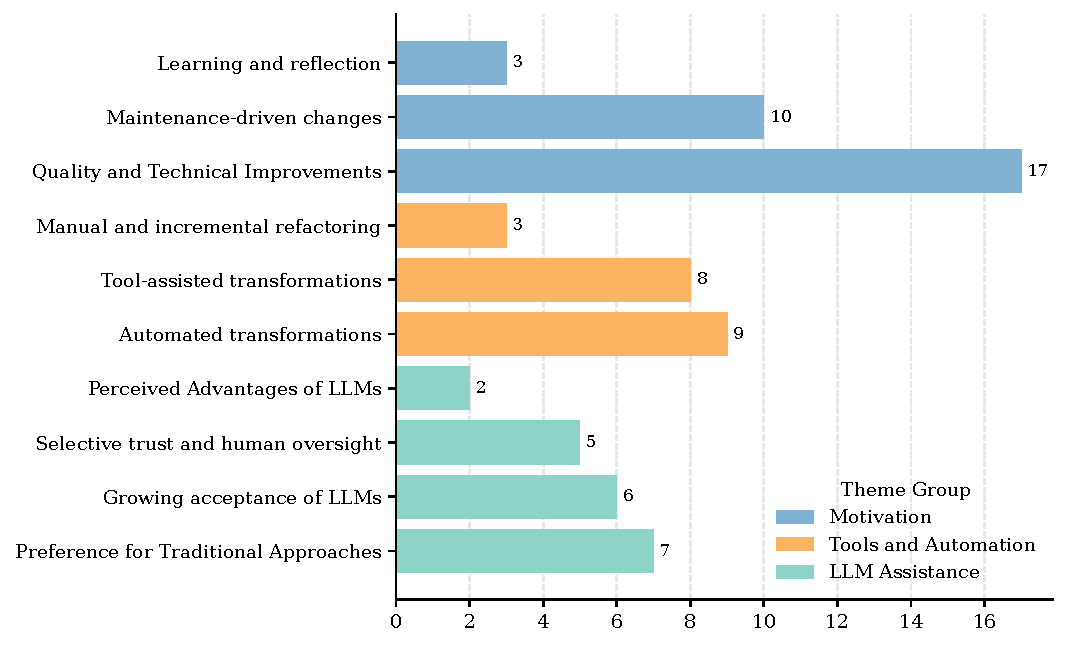
\includegraphics[width=\textwidth]{imgs/rqs_ta.pdf}
\caption{Themes identified from developers' feedback across the three research questions. The numbers represent the frequency of quotations assigned to each theme.}
    \label{fig:motivation_distribution}
\end{figure*}

% This section presents the results of the qualitative investigation conducted to understand the motivations associated with large-scale Type Hint modernization. We first provide an overview of the survey responses obtained from developers responsible for the selected modernization commits, highlighting the main observations. We then present the thematic analysis of the developers feedback, organized according to the three research questions concerning (RQ1) the motivations behind the code changes, (RQ2) the tools and practices employed during the modernization process, and (RQ3) developers perceptions regarding the use of Foundation Models for these tasks. Next, we analyze the corresponding repository artifacts, including commit messages and pull request discussions, to characterize how these motivations and practices are documented in software repositories. Finally, we triangulate both sources of evidence to assess their consistency and identify complementary insights into developers decision-making processes.

\subsection{Overview of Developer Survey Results}

We contacted developers responsible for large-scale modernization commits and then manually validating the candidate commits, we sent 117 emails to developers associated with the recent transformations (2024-2026), while 10 developers were not reachable. Resulting in 107 developers successfully contacted and 20 responses received.

%\todo[inline]{Pessoal, a gente não focou em motivações no estudo anterior. Esse é o foco deste estudo. Alana, pode confirmar isso? Eu lembro de vocês terem olhado os commits / PRs, mas não submetemos tais resultados no paper. Estamos perdendo uma oportunidade aqui neste artigo. E se este trabalho apenas confirma resultados anteriores, ele deixa de ser importante. Eu acho que poderíamos inclusive começar com as análises de Commits / PRs, e usar o survey para complementar as respostas. Como essas mudanças são mais críticas, talvez seja melhor submeter para https://vemworkshop.github.io/vem2026/callForPapers.html. Outra coisa, não estamos evidências que suportam os findings desses parágrafos. Precisamos incluir quotes, links para commits, PRs, etc. Outra opção: https://sbqs.sbc.org.br/2026/index.php/pt/chamada-de-trabalhos/trilha-de-trabalhos-tecnicos}

The reported motivations largely confirm the patterns observed in the mining study. Most developers described the changes as modernization or maintenance activities driven by the evolution of the Python ecosystem, adoption of newer language features, improved readability, better documentation, and stronger static analysis support (\textsc{FastAPI} project -- commit \texttt{3da206c},
\textsc{aiohttp} project -- commit \texttt{35754d4},
\textsc{Wagtail} project -- commit \texttt{80b1ebe})

This is reflected in statements such as:
\begin{quote}
\textit{``Better readability and more expressive code was the main motivation for this change.''} (\textsc{Wagtail} project, commit \texttt{80b1ebe})
\end{quote}

and

\begin{quote}
\textit{``The motivation was due to the deprecation of Python 3.9.''} (\textsc{FastAPI} project, commit \texttt{3da206c})
\end{quote}

Several respondents also highlighted defect prevention and long-term maintainability as important benefits of Type Hints (\textsc{Chia Blockchain} project, commit \texttt{a447734}, \textsc{django-cms} project, commit \texttt{1efaa98}, \textsc{AutoGPT} project, commit \texttt{e16e69c}). For instance:
\begin{quote}
\textit{``This makes the code more resilient against bugs.''} (\textsc{Chia Blockchain} project, commit \texttt{a447734})
\end{quote}

Automation played a central role in many modernization efforts. Developers frequently reported using tools such as \texttt{pyupgrade}, \texttt{ruff}, \texttt{mypy}, and IDE-assisted search-and-replace mechanisms to perform repetitive changes (\textsc{Tornado} project, commit \texttt{113cf79}, \textsc{PyTorch Vision} project, commit \texttt{a095de1}, \textsc{mypy} project, commit \texttt{6682563}).

This is supported by statements such as:
\begin{quote}
\textit{``This commit was generated as part of automated transformations using pyupgrade.''} (\textsc{Tornado} project, commit \texttt{113cf79})
\end{quote}

However, nearly all respondents emphasized the need for manual inspection after automated transformations, particularly in large-scale commits, due to concerns about incorrect modifications and unintended side effects (\textsc{CVAT} project, commit \texttt{5ddeda3}, \textsc{freqtrade} project, commit \texttt{f369151}).

Opinions regarding Foundation Models were more diverse. Some developers viewed LLMs as potentially useful for repetitive typing-related tasks and reported positive experiences using them for code transformations (\textsc{Deep Agents} project, commit \texttt{d398a1e}, \textsc{Pipecat} project, commit \texttt{c4dbe92}). For example:
\begin{quote}
\textit{``Virtually everyone is using agents / LLMs these days for coding.''} (\textsc{Deep Agents} project, commit \texttt{d398a1e})
\end{quote}

and
\begin{quote}
\textit{``Claude Code did almost everything right, but I had to manually edit a few things.''} (\textsc{Pipecat} project, commit \texttt{c4dbe92})
\end{quote}

Others expressed concerns about reliability, predictability, and loss of control over generated changes, preferring deterministic tools for large-scale refactoring activities (\textsc{Wagtail} project, commit \texttt{80b1ebe}, \textsc{Locust} project, commit \texttt{9341cf9}, \textsc{Scrapy} project, commit \texttt{6ecc9e0}).

Finally, the responses are consistent with an important finding from our quantitative analysis: although many Type Hint transformations are mechanical and highly automatable, successful modernization still depends on developer supervision and project-specific decisions (\textsc{Manim} project, commit \texttt{8773252}).

% \todo[inline, color = green]{Essa Seção 5.1 parece mais um resumo dos achados. Uma opção é indicarmos no título da seção que aqui apresentamos apenas um overview das respostas.}

\subsection{Thematic Analysis of Developer Responses}

% \todo[inline, color=green]{TODO: Adicionar hashs dos commits citados}
% \todo[inline, color=green]{TODO: Retirar nome dos autores}
%\todo[inline]{Verificar qual melhor formato para os quotes}
% \todo[inline]{TODO: Adicionar informações, por exemplo, quantas transformações existiam no commit que motivou o contato com o dev.}


\subsubsection{Motivations for Code Changes}
The thematic analysis revealed that large-scale type-related transformations were primarily motivated by quality and technical improvements ($n = 17$). Developers frequently associated these changes with the adoption of modern Python practices, improved readability and maintainability, better IDE support, enhanced static analysis capabilities, and the prevention of subtle bugs. Other responses emphasized architectural concerns, such as reducing code duplication, introducing type abstractions, and addressing limitations in legacy designs. For example, a developer from the \textsc{Wagtail} project (commit ~\texttt{80b1ebe}) explained that adopting newer language features:

\begin{quote}
\textit{``would make the code more readable and expressive''} (\textsc{Wagtail} project, commit ~\texttt{80b1ebe}).
\end{quote}

while a contributor to (\textsc{Chia Blockchain} project, commit ~\texttt{a447734}) noted that the changes were intended to make the code:

\begin{quote}
\textit{``more resilient against bugs''} ( \textsc{Chia Blockchain}, commit ~\texttt{a447734}).
\end{quote}
Maintenance-driven changes represented the second most common motivation theme ($n = 10$). These responses were predominantly associated with the evolution of the Python ecosystem, including the discontinuation of support for older Python versions and dependency maintenance requirements. One respondent from the \textsc{PyTorch Vision} project (commit ~\texttt{a095de1}) explicitly stated that the change was motivated by:

\begin{quote}
\textit{``the motivation was due to the deprecation of Python 3.9.''} (\textsc{PyTorch Vision} project, commit ~\texttt{a095de1})
\end{quote}

whereas another contributor described the modifications as routine maintenance activities. In some cases, ecosystem pressures and quality concerns appeared simultaneously. For instance, a developer from the \textsc{Wagtail} project (commit ~\texttt{80b1ebe}) reported that support for Python 3.8 was being dropped due to its end-of-life status, while newer language features were adopted to improve code quality.

Finally, a small number of responses highlighted learning and reflection as motivations for modernization efforts ($n = 3$). Developers described these transformations as opportunities to gain familiarity with the codebase, improve their understanding of Python typing, and reflect on previous design decisions. 
A developer from the \textsc{Manim} project (commit ~\texttt{8773252}) noted that:
\begin{quote}
\textit{``Adding type annotations allowed me to learn about the source code ... improve my skills related type annotations in python.''} (\textsc{Manim} project, commit \texttt{8773252}).
\end{quote}

% Henrik Skov Midtiby\todo{Melhor ocultar o nome.} in the project Manim, noted that ``Adding type annotations allowed me to learn about the source code" and ``improve my skills related type annotations in python.".

% Other motivations appeared less frequently, including \textit{Bug Prevention} ($n=2$), \textit{Learning and Familiarization with the Source Code} ($n=1$), and \textit{Fixing Typing Issues Caused by Decorators} ($n=1$).

Overall, these findings suggest that large-scale modernization efforts are driven by a combination of internal quality concerns and external ecosystem pressures, while compatibility and maintenance requirements often trigger modernization efforts, developers also perceive these changes as opportunities to improve code quality, simplify architectures, and strengthen the long-term maintainability of their projects.

% Figure~\ref{fig:motivation_distribution} summarizes the distribution of motivations identified through thematic analysis, highlighting the predominance of ecosystem evolution and code quality related factors.

\subsubsection{Refactoring Tools and Practices}

Regarding the transformation practices employed, we observe a strong reliance on automation for large-scale refactorings ($n = 9$). Developers described the use of deterministic tools and scripts, including \texttt{pyupgrade}, \texttt{ruff}, \texttt{sed}, and custom automation scripts, especially in version migration and syntactic modernization tasks. These tools enabled deterministic and repeatable transformations across multiple files simultaneously. (e.g., \textsc{Tornado} project, commit \texttt{113cf79}, \textsc{FastAPI} project, commit \texttt{3da206c}, \textsc{Wagtail} project, commit \texttt{80b1ebe}, \textsc{aiohttp} project, commit \texttt{35754d4}, \textsc{PyTorch Vision} project, commit \texttt{a095de1}, \textsc{pipenv} project, commit \texttt{d6dc5a0}).

\begin{quote}
\textit{``This commit was part of a series of pyupgrade-driven changes... I’d rather use a deterministic tool than an LLM.''} (\textsc{Tornado} project, commit \texttt{113cf79})
\end{quote}

Tool-assisted transformations were also commonly reported ($n = 8$), where developers relied on conventional development tools, such as IDE functionalities, search-and-replace operations, reference updates and utilities such as \texttt{grep}. These tools supported developers carrying out and validating modifications. (e.g., \textsc{AutoGPT} project, commit \texttt{e16e69c}, \textsc{Chia Blockchain} project, commit \texttt{a447734}, \textsc{CVAT} project, commit \texttt{5ddeda3}, \textsc{Roboflow Supervision} project, commit \texttt{fd1277f}, \textsc{mypy} project, commit \texttt{6682563}).

\begin{quote}
\textit{``I probably used VSCode’s find/replace all feature, but no AI tools in this instance.''} (\textsc{AutoGPT} project, commit \texttt{e16e69c})
\end{quote}

Finally, a smaller number of responses ($n = 3$) emphasized incremental refactoring practices. Developers described performing gradual and manual transformations with no tool support. This approach was commonly adopted to cope with architectural constraints and to reduce the risks associated with large-scale modifications. (e.g., \textsc{Manim} project, commit \texttt{8773252}, \textsc{Scrapy} project, commit \texttt{6ecc9e0}, \textsc{Locust} project, commit \texttt{9341cf9}).

\begin{quote}
\textit{``I go file by file, fixing a few type errors at a time and re-running the type checker repeatedly until convergence.''} (\textsc{Manim} project, commit \texttt{8773252})
\end{quote}
\subsubsection{Perceptions of Large Language Model Usage}

With respect to the use of foundation models, the responses reveal a predominance of skeptical or restrictive views regarding their application to simple or deterministic refactoring tasks ($n = 7$). This is reflected in statements such as:

\begin{quote}
\textit{``As long as pyupgrade is maintained, I'd rather use a deterministic tool than an LLM.''} (\textsc{Tornado} project, commit \texttt{113cf79}).
\end{quote}

\begin{quote}
\textit{``That's not something we need LLMs for - it's a straightforward rule-based replacement.''} (\textsc{Freqtrade} project, commit \texttt{f369151}).
\end{quote}

These findings suggest that developers often view type-related transformations as tasks that are already well supported by established tooling ecosystems.

% Furthermore, a set of cases demonstrated an explicit preference for manual approaches over the use of LLMs (n = 2), particularly in scenarios involving large-scale modifications or situations in which developers assume significant responsibility for code correctness. In such contexts, manual control is perceived as more reliable than probabilistic automation, especially when changes affect multiple files or core abstractions. This is illustrated by concerns such as, ``I don't trust an LLM with that'' (in an email response by Matthias, Freqtrade project) and, ``No, I don't believe they are suitable for doing thousands of one-line changes rather than doing them manually'' (in an email response by Tomaz, Locust project).

% The analysis also identified cases of rejection of LLM usage for simple or rule-based tasks (n = 2), reinforcing the perception that such operations do not benefit from probabilistic approaches and are already sufficiently handled by existing deterministic tooling ecosystems, as explicitly stated in "Not for this, it's deterministic and already codified'' (in an email response by the author, Pipenv project).

Despite this preference for conventional approaches, several responses reflected a growing acceptance of LLM-assisted development ($n = 6$). Some developers reported having successfully employed tools such as Claude Code for modernization tasks, whereas others anticipated relying more heavily on language models or coding agents in future refactoring activities. One participant remarked that:

\begin{quote}
\textit{``virtually everyone is using agents / LLMs these days for coding''} (\textsc{Deep Agents project}, commit ~\texttt{d398a1e}).
\end{quote}

While another stated that, if performing the same transformation today, they would 

\begin{quote}

\textit{``100\% use a language model''} (\textsc{Chia Blockchain project}, commit ~\texttt{a447734}).
\end{quote}


A set of responses emphasized selective trust and human oversight ($n = 5$). including the occasional use of tools such as Claude Code. In these cases, developers described using LLMs primarily for consultation or guidance rather than directly incorporating generated code into pull requests. Even when positive experiences were reported, respondents highlighted the need for manual inspection and correction. For instance, one developer noted that 
\begin{quote}
\textit{``Claude Code did almost everything right, but I had to manually edit a few things''} (\textsc{Pipecat}, commit ~\texttt{c4dbe92}).
\end{quote}
illustrating a cautious approach toward AI-assisted development.

Finally, a few responses highlighted specific advantages of LLMs ($n = 2$), particularly for transformations involving semantic understanding rather than purely mechanical replacements. In such cases, developers considered LLMs more convenient than traditional tools and envisioned their application to broader migration tasks where deterministic rules are insufficient.

Overall, the findings suggest that the adoption of LLM for large-scale type-related refactorings is not determined by awareness of the technology itself, but rather by concerns related to predictability, verification overhead, and integration with established deterministic toolchains. Consequently, LLMs are currently positioned as a potential complementary tool to support development workflows, but not replace existing rule-based refactoring pipelines.

\subsection{Thematic Analysis of Repository Artifacts}
We also conduct a thematic analysis of repository artifacts, such as commit messages and pull request discussions related to the 20 survey feedback received. The results reveals that repository artifacts primarily emphasize three complementary aspects of large-scale type hint modernization: the motivations that trigger migration efforts, the technical outcomes produced by these changes, and the strategies adopted to perform them, as shown in Figure~\ref{fig:motivation_distribution_artifacts}.

Regarding motivations, most evidence falls under \textit{Modernization Infrastructure} ($n = 10$). Repository discussions frequently associate large-scale transformations with broader maintenance initiatives, such as dropping support for legacy Python versions, adopting newer language features, enabling static analysis tools or aligning the codebase with updated development practices. Rather than presenting type annotations as isolated improvements, developers often describe them as part of larger modernization campaigns affecting the entire project infrastructure.

The analysis of outcomes shows that repository discussions primarily focus on the resulting evolution of the type system, with \textit{Type System Evolution} accounting for 19 quotations. Pull request conversations frequently discuss the technical consequences of the migration, including improvements in type inference, static checking, compatibility with modern typing syntax, and the resolution of typing inconsistencies. This emphasis is reflected in comments such as:

\begin{quote}
\textit{``This is mostly typing changes, to use built-in functionality instead of imports from the \texttt{typing} module.''} (\textsc{Tornado} project, PR \texttt{\#3596})
\end{quote}

This predominance reflects the collaborative nature of pull request reviews, where developers spend more effort discussing the correctness and implications of typing decisions than the motivations behind the migration itself.

Finally, the identified strategies indicate that modernization efforts are rarely performed through isolated edits. Most quotations describe coordinated migration strategies, again concentrated in \textit{Modernization Infrastructure} ($n = 14$), such as repository-wide automated rewrites, the adoption of tools like \texttt{pyupgrade}, systematic migration to newer typing syntax, and project-wide cleanup after dropping support for older Python versions. One representative example explicitly describes this workflow:

\begin{quote}
\textit{``Update type annotations with py3.8 features. Automated change with \texttt{pyupgrade} (restricted to the typing plugins), followed by manual removal of unused imports.''} (\textsc{Tornado} project, commit \texttt{113cf79})
\end{quote}

Additional strategies involve code restructuring and API redesign ($n = 6$), suggesting that type hint modernization is frequently performed alongside broader refactoring activities.

Overall, these findings suggest that large-scale type hint transformations are embedded within broader software evolution initiatives. While the initial motivation is commonly driven by infrastructure modernization and ecosystem evolution, repository discussions predominantly concentrate on ensuring the technical correctness of the resulting type system. This observation complements the evidence obtained from developers' responses by showing more technical discussions about how modernization migrations are implemented and the collaborative review process.

\begin{figure}[!h]
    \centering
    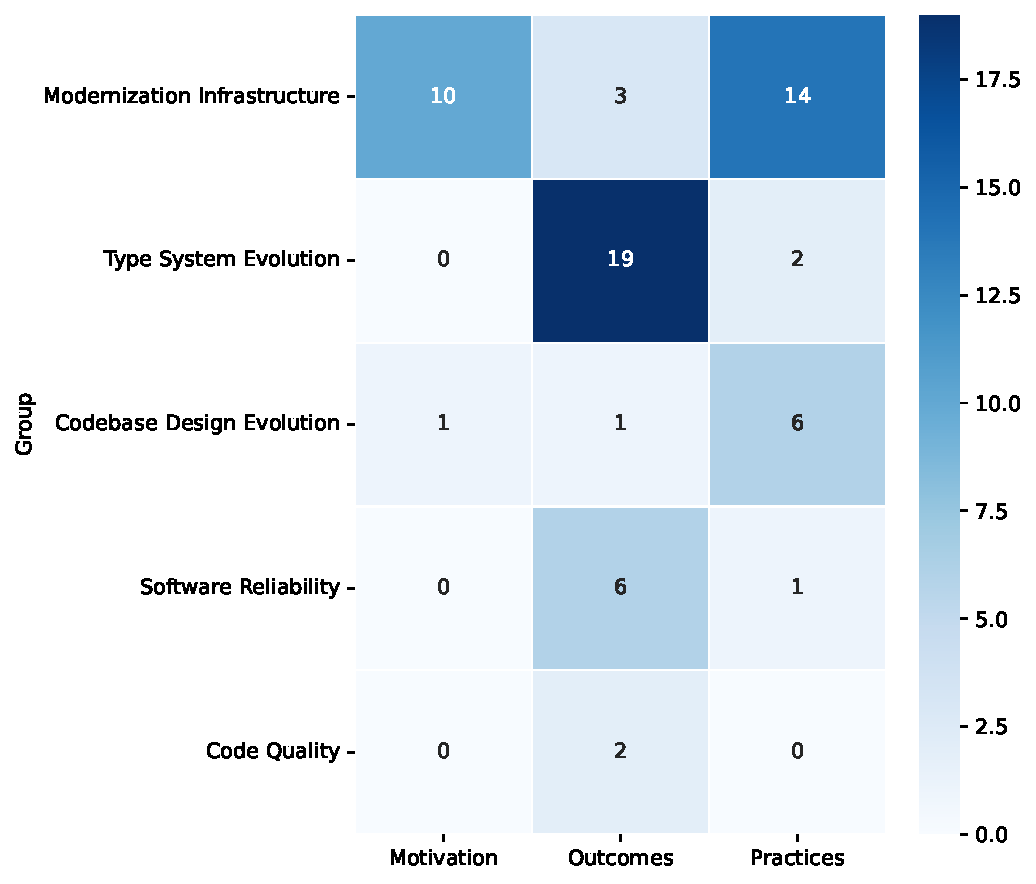
\includegraphics[width=\columnwidth]{imgs/artifacts_ta.pdf}
    \caption{Themes identified from repository artifacts analysis.}
    
    \label{fig:motivation_distribution_artifacts}
\end{figure}

\subsection{Triangulation Results}

\begin{figure*}[!t]
    \centering
    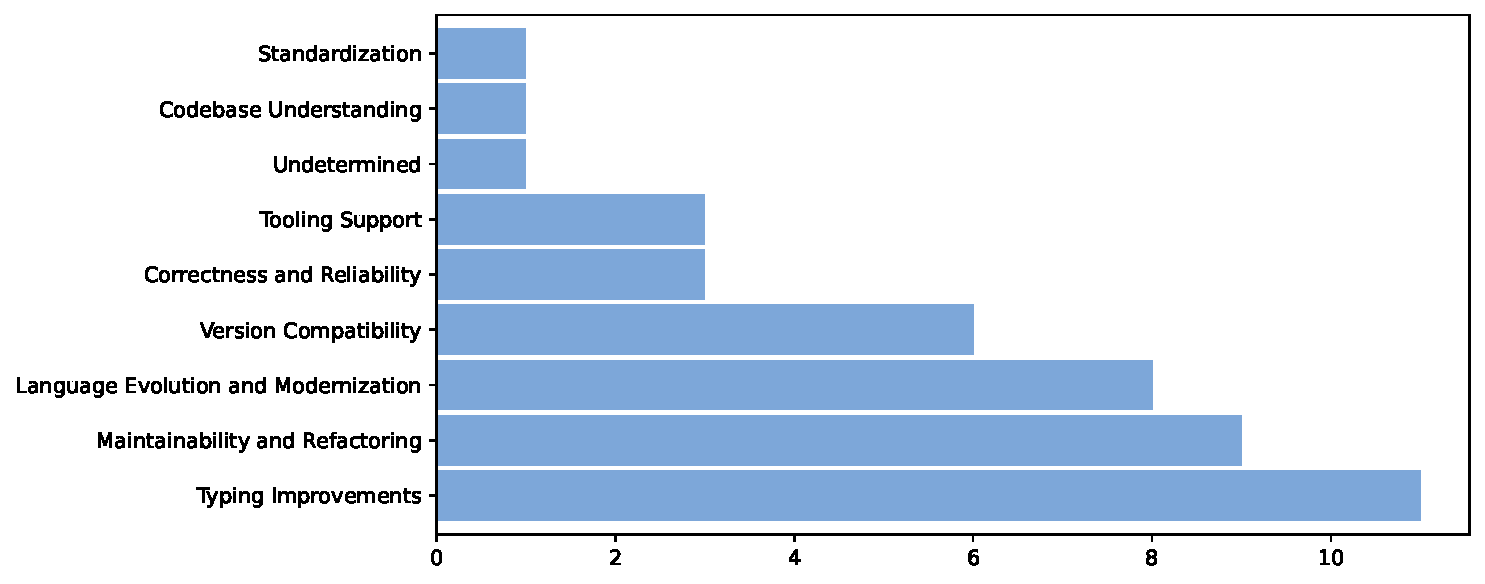
\includegraphics[width=\textwidth]{imgs/triangulation.pdf}
    \caption{Frequency of motivation categories identified across the triangulated cases.}
    \label{fig:triangulation}
\end{figure*}

To assess the consistency between available repository artifacts and developers' feedback, we compared the themes identified from commit messages, pull request discussions, and code review comments with those obtained from the survey responses. Overall, the triangulation revealed a high level of agreement between both sources. 85\% of the analyzed cases demonstrated at least partial convergence regarding the motivations behind the modernization effort.

Beyond validating the consistency of the findings, the triangulation also showed that the two sources provide complementary perspectives on the same development activity, as shown in Figure~\ref{fig:triangulation}. Repository artifacts primarily document the technical rationale of the changes, emphasizing modernization campaigns, Python version migrations, tooling adoption, and implementation strategies. In contrast, survey responses more frequently expose the developers' decision-making process, highlighting perceived benefits such as improved readability, maintainability, type safety and code quality. Consequently, both sources differ in the level of abstraction and the aspects they emphasize.

Across the cases, the most recurrent motivation categories were Typing Improvements ($n=11$), Maintainability and Refactoring ($n=9$), Language Evolution and Modernization ($n=8$), and Compatibility ($n=6$). Less frequent themes included Correctness and Reliability ($n=3$), Tooling Support ($n=3$), Standardization ($n=1$), Codebase Understanding ($n=1$), and one case classified as Undetermined. These categories closely match the dominant themes independently identified in both thematic analyses, reinforcing that large-scale type hint modernization is primarily motivated by software quality improvements, adoption of evolving Python language features, and long-term maintenance concerns rather than isolated code changes.

The observed convergence increases confidence that repository artifacts provide a reliable approximation of developers' motivations in large-scale modernization efforts. At the same time, the survey responses reveal contextual information that is rarely documented in commits and pull request discussions, suggesting that combining both sources produces a richer understanding of developer intent than relying on either source alone.

% The analysis of the 20 commit--pull request--email sets revealed a generally high degree of consistency across the three sources. Overall, most cases showed that the intent behind software changes was similarly expressed across commit messages, pull request descriptions, and email responses.

% In a qualitative assessment of consistency, the majority of cases were classified as exhibiting high consistency, where the same underlying motivation or objective could be clearly identified across all three artifacts. A smaller number of cases showed moderate consistency, typically due to differences in the level of detail or emphasis across sources. Only a few cases exhibited low consistency, generally associated with missing or less explicit information in one of the artifacts, rather than direct contradictions.

% Regarding the identified categories, transformations related to language evolution and code modernization were the most prevalent. These changes include, for example, the adoption of new language constructs, updates to syntax in newer Python versions, and the incorporation of features such as \ths. This category reflects the use of newer language functionalities and the continuous updating of coding standards.

% Next, changes aimed at improving type safety stand out, involving the introduction or refinement of type annotations to reduce potential runtime errors. This category is associated with strengthening the type system and the adoption of gradual static typing within the Python ecosystem.

% Categories such as refactoring, compatibility, standardization, and tooling improvements appeared less frequently, suggesting that most transformations are more strongly associated with language ecosystem evolution than with deep structural code reorganizations or infrastructure-level adjustments.

% The comparison across sources also revealed a clear division of roles in documenting software changes. Commits tend to record operational aspects of the implementation, pull requests provide a broader view of the underlying technical objectives of the transformation, and emails often contribute organizational context and decision-making rationale.

% Taken together, these results indicate that the three sources represent complementary levels of expressing change intent, reinforcing the importance of artifact triangulation for a more comprehensive understanding of the motivations associated with software rejuvenation.

% �� Commits (hash curto)
% Tornado
% 113cf79
% FastAPI
% 3da206c
% Deep Agents (LangChain AI)
% d398a1e
% Django CMS
% 1efaa98
% aiohttp
% 35754d4
% CVAT
% 5ddeda3
% AutoGPT (OpenAI ecosystem project)
% e16e69c
% PyTorch Vision
% a095de1
% LlamaIndex
% e157ebb
% Pipecat
% c4dbe92
% Roboflow Supervision
% fd1277f
% Manim Community
% 8773252
% Freqtrade
% f369151
% Reflex
% 25016f5
% Pipenv
% d6dc5a0
% Wagtail
% 80b1ebe
% Locust
% 9341cf9
% Chia Blockchain
% a447734
% mypy
% 6682563
% Scrapy
% 6ecc9e0

\section{Discussion}
\label{sec:discussion}
This section discusses the implications of our findings in light of the research questions. We interpret the evidence obtained from the developer survey, repository artifacts, and their triangulation to better understand the motivations of developers performing large-scale Type Hint modernization, the practices adopted that support large-scale transformations and the developers perception of Foundation Models in supporting such activities.

\subsection{RQ1: \textit{What motivations drive developers to perform large-scale Type Hint modernization efforts?}}

Our findings suggest that large-scale Type Hint modernization is driven by the interplay between ecosystem evolution and software quality objectives. Although many modernization campaigns are initiated in response to changes in the Python ecosystem, developers consistently associate these transformations with expected benefits to code quality, including improving maintainability, readability, static analysis support, and reducing the likelihood of defects.

This interpretation is reinforced by the convergence of evidence across repository artifacts and developer feedback. Commit messages and pull request descriptions frequently emphasize the technical aspects of the modernization process, such as migrating to newer typing syntax, updating compatibility with recent Python versions and and tooling adoption. In contrast, developers responses reveal the broader motivations underlying these changes related to quality and maintainability.

These findings complement previous repository-mining studies by providing insight into the motivations behind large-scale modernization efforts. Our results suggest that Type Hint modernization is perceived as part of long-term software evolution, where ecosystem changes act as triggers for improvements, while developers leverage these opportunities to introduce improvements that strengthen software evolution.

\subsection{RQ2:\textit{What tools or automation techniques do developers use to support large-scale Type Hint modifications?}}

Our results reveal that deterministic automation tools are broadly used for executing large-scale modernization. Tools such as pyupgrade, ruff, IDE-assisted refactorings, and custom scripts enable developers to perform thousands of type-related transformations.

However, the usage of deterministic automation tools is not perceived as a fully autonomous process. We also note a concern with ensuring that large-scale transformations are verified, as well as a focus on deterministic tools that guarantee deterministic behavior. Automation is consistently accompanied by manual verification. Rather than delegating the entire modernization process to tools, developers described workflows in which automated transformations generate candidate modifications that are subsequently reviewed and validated before integration.

This observation helps explain how developers performing large-scale type-related transformations. These modernizations appears to dependent less on manually individual editing than on selecting reliable transformations tools and ensuring that works correctly, where deterministic automation performs repetitive transformations while developers remain responsible for validating semantic correctness and project-specific decisions.

\subsection{RQ3:\textit{How do developers perceive the potential use of Foundation Models to assist Type Hint modernization tasks?}}

Our results suggest a growing openness among developers to incorporate Foundation Models into their modernization workflows, but not yet as replacements for deterministic transformation tools. While several participants reported positive experiences using LLMs for programming tasks and anticipated an increasing role for AI-assisted development, they also expressed reservations regarding the reliability, predictability, and verification of large-scale automated changes.

There is a temporal aspect that helps explain the coexistence of seemingly contrasting themes identified in the analysis. While deterministic tools remain the preferred choice for large-scale mechanical transformations, developers also reported growing confidence in Foundation Models and increasingly viewed them as viable assistants for future modernization efforts. Rather than representing conflicting opinions, these responses are consistent with an ongoing technological transition in which AI-assisted development is progressively becoming part of software engineering practice.

Although deterministic automation remains the dominant approach for large-scale Type Hint modernization, the reported growing acceptance of Foundation Models suggests that modernization workflows are likely to become increasingly hybrid and perceived as valuable for supporting activities that require contextual understanding, planning or developer assistance.


\section{Threats to Validation}
\label{sec:threats}
Throughout this study, we consider that our methods were effective in supporting the analysis of refactoring practices related to Type Hint adoption and software modernization in Python projects. However, several limitations may influence the interpretation of the results.

In this work, we operationalize the concept of software rejuvenation as refactoring activities related to the adoption of Type Hints. Although this definition captures an important aspect of modernization in the Python ecosystem, it represents only a partial view of the broader concept of software rejuvenation, not covering other forms of code evolution and improvement.

In addition, the dataset is restricted to open-source Python projects hosted on GitHub, selected based on activity and maturity criteria. While this enables the analysis of relevant and actively maintained systems, it may introduce a bias toward more established repositories, limiting generalization to smaller projects, other programming languages, or industrial contexts. The data selection process may also introduce sampling bias, since we focused on commits with a large number of detected transformations and selected one representative commit per developer, which may overrepresent large-scale modernization efforts and underrepresent incremental changes.

Regarding data collection, we relied on GitHub APIs to extract commits, pull requests, and associated discussions. Although this ensures reproducibility, platform limitations such as incomplete metadata and the absence of external communication channels may affect the full reconstruction of development context.

Since this study uses thematic analysis, there is an inherent risk of interpretative bias, as different researchers may code the same data in different ways. To mitigate this risk, we adopted independent coding, iterative refinement of the codebook, and consensus-based discussion, although some degree of subjectivity remains unavoidable due to the qualitative nature of the analysis.

Additionally, the survey introduces self-selection and response bias, as participation was voluntary and only 20 out of 117 contacted developers responded (17.09\% response rate). This may limit the representativeness of the sample, as responses may be skewed toward developers more engaged with or interested in Type Hint modernization. Recall bias may also affect how developers report past decisions, potentially influencing response accuracy.

Finally, the results reflect a specific temporal window of the Python ecosystem. Given the rapid evolution of development tools, especially with the increasing adoption of LLM-based systems, the findings should be interpreted as representative of the observed period rather than a stable characterization of current or future practices.


%\section{Threats to Validation}

\section{Conclusion}
\label{sec:conclusion}
This study investigated the motivations, decision-making process, and perceived role of Foundation Models in large-scale Type Hint modernization by combining repository mining, developer surveys, and qualitative thematic analysis. We found that these efforts are primarily driven by software maintainability, improvements to type information, Python language evolution, and compatibility requirements. The triangulation of repository artifacts and developer feedback revealed a high degree of consistency across data sources while also demonstrating their complementary nature: repository artifacts capture the technical aspects of modernization, while developers provide additional insight into the underlying rationale and decision-making process.

Our findings further show that large-scale Type Hint modernization is commonly supported by automation, with developers relying on specialized tools while reserving manual effort for validation and project decisions. Although Foundation Models were rarely used in the analyzed cases, most participants viewed them as promising assistants for repetitive modernization tasks, provided that human oversight is maintained. These results contribute to a better understanding of the factors driving large-scale Type Hint modernization and highlight the emerging interest in the use of Foundation Models to support these activities, motivating further research on AI-assisted modernization techniques.

\section*{Acknowledgements}
<text included by the authors>

%% The next two lines define the bibliography style to be used, and
%% the bibliography file.
\bibliographystyle{ACM-Reference-Format}
\bibliography{bibliography}

\end{document}

% ============================================================
% CBSoft ACM-like Template – Author Checklist
% ============================================================
%
% 1. Remove CCS Concepts
%    - Remove the CCSXML block and \ccsdesc commands.
%
% 2. Remove ACM footer
%    Use the command \renewcommand\footnotetextcopyrightpermission[1]{}
%
% 3. Remove ACM Reference Format
%    Use the commands \setcopyright{none} and 
%    \settopmatter{printacmref=false}
%
% 4. Short title must not exceed column width
%    Use the command 
%    \renewcommand{\shorttitle}{The Name of the Title Is Hope}
%
% 5. Include authors' surnames in the page headers (even pages)
%    - The author names in the page header (at the top of the page)
%      must not exceed the column width
%    - This list must contain only the authors' surnames
%    - Suggestion: use "Surname et al." for more than two authors with the
%      command \renewcommand{\shortauthors}{Surname1stAuthor et al.}
%
% 6. Author format below title:
%    \author{FirstName Surname}
%    \affiliation{
%      \institution{Department, Institution}
%      \city{City}
%      \country{Country}}
%    \email{email@email.com}
%
% 7. Verify all author emails are included
%    - Check font consistency
%
% 8. All numbered section and subsection titles must follow the same
%    capitalization style: the first letter of each word in the title 
%    must be capitalized (Title Case).
%
% 9. Artifact Availability (check CFP)
%    - Not numbered -- use \section*{Artifact Availability}
%    - Placed after Conclusion and before Acknowledgments
%    - In Portuguese, use \section*{Disponibilidade de Artefatos}
%
% 10. Abstract
%     - Single paragraph
%     - Papers written in Portuguese must use "Resumo" instead of "Abstract"
%       with the command \renewcommand\abstractname{Resumo}
%
% 11. Keywords
%     - Comma-separated, first letter capitalized
%     - Papers written in Portuguese must use "Palavras-chave" instead of
%       "Keywords" with the command 
%       \renewcommand\keywordsname{Palavras-chave}
%
% 12. References
%     - Not numbered -- already enforced by the template
%     - Papers written in Portuguese must use "Referências" instead of
%       "References" with the command \renewcommand\refname{Referências}
%
% 13. Acknowledgements
%     - Optional section
%     - Not numbered -- use \section*{Acknowledgements}
%     - In Portuguese, use \section*{Agradecimentos}
%
% 14. Remove received/revised/accepted dates
%
% 15. Figure captions must appear below figures
%
% 16. Verify the symposium name in the page header
%    - Use English, even if the paper is written in Portuguese
%    - Select the correct event according to the track
%    - Use Arabic ordinal numbers, not Roman
%
%    SBES (Research, Education, IIER, Tools, Industry)
%    \acmConference[SBES 2026]{40th Brazilian Symposium on Software Engineering}{September 8--11, 2026}{São Paulo, SP, Brazil}
%
%    SBLP
%    \acmConference[SBLP 2026]{30th Brazilian Symposium on Programming Languages}{September 8--11, 2026}{São Paulo, SP, Brazil}
%
%    SBCARS
%    \acmConference[SBCARS 2026]{20th Brazilian Symposium on Software Components, Architectures, and Reuse}{September 8--11, 2026}{São Paulo, SP, Brazil}
%
%    SAST
%    \acmConference[SAST 2026]{11st Brazilian Symposium on Systematic and Automated Software Testing}{September 8--11, 2026}{São Paulo, SP, Brazil}
%
%    Workshops
%    \acmConference[Workshop Acronym 2026]{Workshop Full Name}{Workshop Date}{São Paulo, SP, Brazil}
%
%
% 17. Remove colored author names, citations, and links
%
% 18. Camera-ready only:
%     Do not use the "review" or "anonymous" modes in the 
%     \documentclass command
%
% 19. SBES Tools Track papers must include a demo video link at the end of
%     the abstract
%     Example:
%     \begin{abstract}
%     <abstract text> \newline
%     \textbf{Demo video:} <video link>
%     \end{abstract}
%
% 20. SBES Industry Track papers must not include author biographies
%
% ============================================================

\endinput


